\documentclass[../../main.tex]{subfiles}

\begin{document}

\chapter{Implementation}
\label{chap:implementation}

In this chapter, we present the implementation details of \wassis, our prototype developed to explore Wave Function Collapse (WFC) for software system visualization.

\section{Development Environment}

\wassis is implemented in Pharo~\citebibliography{Blac2009a}, a Smalltalk environment. This choice comes from the tradition of Smalltalk in software visualization and software analysis. Various tools such as \tool{Moose}~\citebibliography{Nier2005a}, \tool{CodeCity}~\citebibliography{Wett2007a}, and \tool{CodeCrawler}~\citebibliography{Lanz2003a}, were developed using Smalltalk. This makes Pharo a suitable environment for a software visualization prototype such as \wassis.

In Pharo, everything is an object. This makes it possible to represent the main concepts of \wassis, such as grids, cells, tiles, paths, directly as objects. This keeps the implementation close to the conceptual model.

Finally, Pharo provides an interactive and reflective development environment with integrated inspector, debugging and profiling tools. This was particularly useful for \wassis, as WFC continuously changes the state of cells during execution. For example, individual cells can be inspected to check their possible tiles, entropy, and neighbors during generation. This made it easier to understand and debug the generation process.

\section{Software Architecture}

\wassis is organized into two Pharo packages: \texttt{Wassis-Model}, which contains the core model and the algorithms, and \texttt{Wassis-Visualization}, which is responsible for rendering the results using Roassal~\citebibliography{Berg2022a}. \wassis core architecture is show in \figref{fig:wassis_architecture}.

At the highest level, \texttt{WSAdaptiveSolver} manages the execution process and the grid size. It creates a new \texttt{WSSolver} for each attempt, starting from an initial grid size and increasing it when no valid solution is found. Therefore, each \texttt{WSSolver} represents one execution of WFC on a grid of a fixed size. This separation keeps the WFC algorithm independent of the logic used to increase the grid size during multiple attempts.

\texttt{WSSolver} is the main orchestrator of a single WFC execution. It operates on a \texttt{WSGraph}, which represents the structure on which WFC is executed. The graph is composed of \texttt{WSNode} objects, each representing a cell on the grid. A node stores information such as its  identifier, position, entropy, and, most importantly, a collection of possible \texttt{WSTile} objects (empty, class, and path tiles). Hence, the \texttt{WSGraph}, \texttt{WSNode}, and \texttt{WSTile} classes are the core objects manipulated by WFC.

The topology is represented by \texttt{WSTopology}. It defines the structure of the graph, such as how nodes are arranged on the grid and how neighboring nodes are determined. This abstraction allows WFC to work with different grid structures, such as rectangular and hexagonal grids, without depending on a specific topology.

Contradictions are handled by the \texttt{WSBacktracking} class. Different recovery strategies are implemented as separate classes following the Strategy design pattern, allowing the solver to restore a previous state or restart the execution without modifying its logic. A checkpoint of the graph state is saved using the Memento pattern.

After a successful WFC execution, the result is then passed to the visualization package, which uses Roassal to render the generated grid.

\begin{figure}[ht]
    \centering
    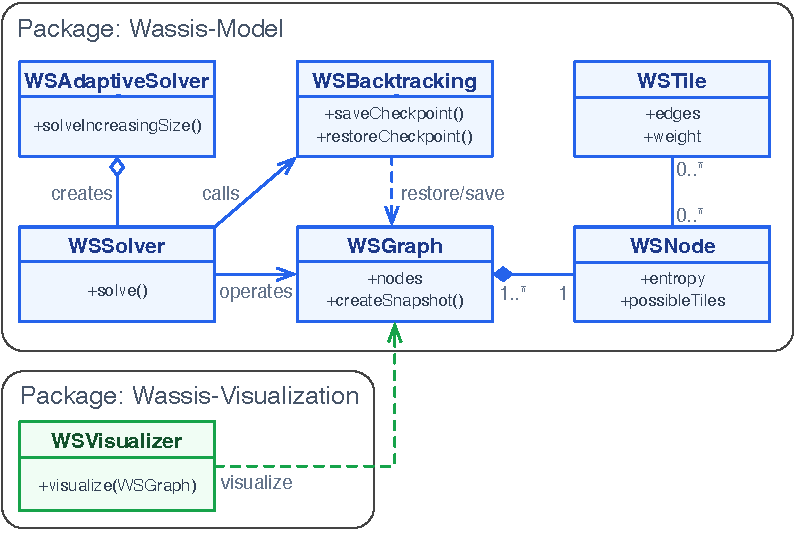
\includegraphics[width=\linewidth]{figures/implementation/architecture}
    \caption{Core Architecture of \wassis}
    \label{fig:wassis_architecture}
\end{figure}

\section{Code Parsing}

The source code parsing is performed using \tool{ZION}, a tool developed within the REVEAL Research Group by Giannaccari~\etal~\citebibliography{Gian2026a}. \tool{ZION} uses CodeQL~\citeonline{CodeQL} to extract software entities, relationships, and properties from a source code repository. The extracted data is stored in a JSON file.

\wassis uses \tool{ZION}'s domain model to load this data and access the extracted entities and relationships. These are then mapped to the internal representation used by \wassis. A \texttt{WSSoftwareSystem} contains the classes of the analyzed system, represented as \texttt{WSClass} objects. Each class stores its incoming and outgoing relationships, which represent its dependencies on other classes. This representation provides the information required by the layout and path generation phases, so the resulting model is used as input for the WFC algorithm.

\subfile{class_layout_placement.tex}
\subfile{wave_function_collapse.tex}

\section{Path Optimization}

\wassis uses Dijkstra's algorithm during the optional path optimization step described in \subsecref{subesc-approach:path_optimization}. Instead of implementing the algorithm from scratch, \wassis uses the \texttt{AIDijkstra} implementation provided by Pharo's \texttt{AIGraphAlgorithm} package.

For direct connections, Dijkstra is used to find the shortest path between the border nodes of two classes. For merged paths, a class must be connected to the existing backbone. Since the class can connect to any node of the backbone, \wassis uses a virtual target node to find the shortest path to the backbone.

The virtual target is an additional node that does not correspond to any grid cell. A directed edge with cost zero is added from every node belonging to the current backbone to this virtual target. Dijkstra is then run from each border node of the class to the virtual target. Since reaching the virtual target has zero cost from every backbone node, the shortest path found corresponds to the shortest path from that border node to the backbone.

The paths obtained from the different border nodes are compared, and the shortest one is selected.

\section{Memory Management}

During WFC generation, \wassis creates many temporary objects, such as graph and node instances, heap entries, and snapshots. Pharo stores all active objects in memory. Therefore, repeated WFC attempts can cause memory usage to grow over time as temporary objects from previous attempts become unused.

To avoid this problem, \wassis runs a garbage collection after each failed attempt that requires a grid expansion. This allows unused objects from the previous attempt to be removed from memory before the next generation starts.

The garbage collection has a small performance cost, but prevents memory usage from increasing indefinitely across multiple WFC attempts.

\section{Parallel Execution}

Pharo is a single thread environment and does not support true multithreading. This is a limitation for \wassis, since running multiple WFC generations in parallel can be useful to obtain different valid solutions and compare their metrics. It can also be used to explore different generation choices, which may lead to different valid or better-looking solutions.

Since true multithreading cannot be used, \wassis uses multiple independent Pharo images to achieve parallel execution. Shell scripts are provided to start multiple instances of the same Pharo image, with each instance running an independent WFC generation. This allows multiple generations to run in parallel without requiring changes to the WFC algorithm to support multithreading.

Two execution modes are available. In the first, all instances run until they complete. Each solution is serialized and saved in a separate folder, so it can be loaded later from another Pharo image. Serialization is implemented using Fuel~\citeonline{LeskeFuel}.

The second mode is designed to find a valid solution as quickly as possible. All instances run simultaneously, and the execution stops when one of them finds a solution. The winning instance sends its process identifier to the shell script through a pipe. The script then terminates the other Pharo processes and opens the winning image to display the solution.

This approach provides parallel execution while keeping each WFC generation single-threaded.

\subfile{tool.tex}

\section{Summary}

This chapter presented the implementation of \wassis, a Pharo prototype for generating software visualizations using the approach described in \chapref{chap:approach}. The implementation is organized into a core package containing the model and algorithms and a visualization package responsible for rendering the results with Roassal. The main execution is managed by a solver, which performs independent WFC executions and increases the grid size when a valid solution cannot be found.

The implementation uses the software system model produced by ZION~\citebibliography{Gian2026a}, which performs the parsing and analysis of the source code to extract classes and their relationships. These entities are mapped to the internal representation of \wassis. Class placement is implemented using metric Multidimensional Scaling (mMDS), followed by a mapping from continuous coordinates to grid positions. Classes are represented using square footprints, whose size is determined by their number of connections. Before WFC starts, the border cells of each footprint are assigned to paths according to their preferred directions, computed using cosine similarity.

The WFC solver introduces various mechanisms to improve performance and making path generation possible. A max-heap is used to efficiently select the cell with the highest entropy, while lazy heap entries and heap compaction reduce the cost of updating the heap during propagation. Placeholder tiles are dynamically resolved during generation to avoid requiring a tile for every possible path. Dynamic tile weights guide paths toward their targets.

Contradictions are handled through backtracking strategies implemented using the Strategy pattern, allowing different recovery strategies to be selected without changing the solver. Checkpoints store only the mutable state needed to restore the grid, using the Memento pattern instead of expensive deep copies. \wassis also provides an optional path optimization step based on Dijkstra's algorithm, which can improve direct and merged paths after WFC generation.

Finally, garbage collection is performed after failed attempts that require grid expansion to prevent memory usage from growing across generations. Since Pharo does not support true multithreading, \wassis runs multiple independent Pharo images to generate solutions in parallel.

The implementation also includes a user interface that allows users to configure the generation, select the input system, and inspect the generated visualization. The tool provides additional views, including the step-by-step WFC animation, metrics dashboard, system graph, classes distance matrix, and MDS placement. These views support both the inspection of the generated solution and the analysis of the generation process.

\end{document}